% UPDATED BY MARCUS SCHAGERBERG, 2023
% CREATED BY WOLFGANG AHRENDT, 2021


\section{Unity}
Unity is a cross-platform game engine used to create both 2D and 3D games. Unity supports a lot of features that speed up development time. 

% WRITTEN BY HANNES KAULIO, 2023
\section{Cubic Bézier Curve}
A cubic Bézier curve is a parametric curve defined by four control points. The four control points define a smooth, continuous curve.

\begin{figure}[!h]
    \centering
    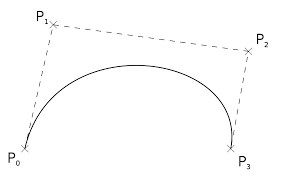
\includegraphics[scale=0.5]{Project_report/figures/bezier-curve.png}
    \caption{Cubic Bézier curve with control points P\textsubscript{0}, P\textsubscript{1}, P\textsubscript{2} and P\textsubscript{3}}
\end{figure}

The cubic Bézier curve can be defined by the formula\cite{Cubic-Bézier-Curves}: \[P(t) = (1-t)^3P_0 + 3t(1 - t)^2P_1 + 3t^2(1 - t)P_2 + t^3P_3, 0 \le t \le 1. \]
Cubic Bézier curves have some basic properties.
\begin{itemize}
    \item 1. P\textsubscript{0} and P\textsubscript{3} are on the curve
    \item 2. The curve is continuous, infinitely differentiable, and the second derivatives are continuous.
    \item 3. The tangent line to the curve at the point P\textsubscript{0} is the line P\textsubscript{0}P\textsubscript{1}. The tangent to the
curve at the point P\textsubscript{3} is the line P\textsubscript{2}P\textsubscript{3}.
    \item 4. Both P\textsubscript{1} and P\textsubscript{2} are on the curve only if the curve is linear.
\end{itemize}

\subsection{Bézier Clipping}

% WRITTEN BY HANNES KAULIO, 2023
\section{Composite Bézier curve}
A composite Bézier curve is a spline made out of Bézier curves. The series of bezier curves are joined together end to end with the start point of one curve coinciding with the end point of the other curve.

% WRITTEN BY HANNES KAULIO, 2023
\section{A* Algorithm}
A* is an algorithm widely used for path finding and graph traversal \cite{A-Star-Algorithm}. Given a start, and end node in a weighted graph, the algorithm will find the shortest path between the nodes. 
\section {Mesh Generation}

\section{ABM}

